\section{实验二\ \ 内存管理}

\subsection{实验目的}
\begin{enumerate}
    \item 了解和掌握操作系统中逻辑地址到物理地址的转换的实现原理。
    \item 了解和掌握操作系统中动态内存分配和回收的处理机制。
    \item 了解操作系统中用户态栈空间的管理,掌握简单与复杂的缺页异常处理方法。
\end{enumerate}

\subsection{实验内容}
\paragraph{lab2_1 虚实地址转换} 本实验仍然是完善printu系统调用。与lab1_1不同之处在于,本实验采用Sv39虚地址管理方案,因此需要执行虚实地址转换方可完成对指定字符串的输出。虚实地址转换是通过user_va_to_pa()函数完成的,该函数的实现需要在实验中进行补充完善。

函数的补充完善可以通过调用页表操作相关函数lookup_pa找到页表page_dir中虚拟地址va对应的pteaddr,再通过计算va在页内的位移,将位移与pteaddr进行拼接,得到va对应的物理地址,函数user_va_to_pa补充的代码如下。
\begin{cppcode}
void *user_va_to_pa(pagetable_t page_dir, void *va) {
    uint64 uint64_va = (uint64)va;
    uint64 pteaddr = lookup_pa(page_dir, uint64_va);
    if(pteaddr == 0) {
        panic( "Invalid va.\n");
        return (void *)NULL;
    }
    else return (void *)(pteaddr + (uint64_va & ((1<<PGSHIFT) -1)));
}
\end{cppcode}
\paragraph{lab2_2 简单内存分配和回收}
动态内存分配和回收是操作系统堆空间管理的内容,本实验已经完成了naive_malloc函数的实现,该函数基于kernel/syscall.c中的sys_user_allocate_page系统调用,通过user_vm_map调用页表操作函数map_pages实现简单的堆空间分配。

本实验需要补充完成naive_malloc的
“逆操作”——naive_free,实现简单的堆空间释放。观察跟踪代码发现,naive_free函数基于sys_user_free_page系统调用,该系统调用又调用了user_vm_unmap函数,该函数需要完善。

堆空间的释放需要遍历需要释放的虚拟地址范围内所有可能的虚拟页面起始地址,通过page_walk函数获取虚地址对应物理页面的pte,若pte有效,则通过pte获取物理地址pa,并使用free_page函数释放该物理页面,同时将pte的有效位置0。user_vm_unmap函数的补充代码如下。

\begin{cppcode}
void user_vm_unmap(pagetable_t page_dir, uint64 va, uint64 size, int free) {
    uint64 first, last;
    void *pa;
    pte_t *pte;
    for (first = ROUNDDOWN(va, PGSIZE), last = ROUNDDOWN(va + size - 1, PGSIZE);
         first <= last; first += PGSIZE, pa += PGSIZE) {
        pte = page_walk(page_dir, first, 0);
        if (pte) {
            pa = (void *) PTE2PA(*pte); // get physical address
            if (free) free_page(pa);    // free page
            *pte &= (~PTE_V);           // invalidate pte
        }
    }
}
\end{cppcode}
\paragraph{lab2_3 缺页异常} 实验需要支持一个较为庞大的函数递归调用过程,该过程会占满用户栈空间,从而引发缺页异常。本实验需要完善用户态栈空间的管理,使得系统能够正确处理用户进程的“压栈”请求。通过阅读delegate_traps()函数,得知缺页异常(CAUSE_STORE_PAGE_FAULT)已经代理给了S模式,因此需要在kernel/strap.c文件中执行对于这类异常的处理。

在kernel/strap.c中,smode_trap_handler函数中包含对CAUSE_STORE_PAGE_FAULT和CAUSE_LOAD_PAGE_FAULT两种缺页异常的处理,相应的处理函数均为handle_user_page_fault。由于本实验涉及的是写入栈的缺页异常,因此只需完善handle_user_page_fault函数中的CAUSE_STORE_PAGE_FAULT情况即可。解决缺页异常首先需要使用alloc_page函数分配一个新的物理页面,然后使用prot_to_type函数将permission code转换为PTE的permission type,即为页面设置合适的权限,最后使用user_vm_map执行虚拟页面到物理页面的映射,即完成一次缺页异常的处理。handle_user_page_fault函数的实现如下。
\begin{cppcode}
void handle_user_page_fault(uint64 mcause, uint64 sepc, uint64 stval) {
    sprint("handle_page_fault: %lx\n", stval);
    switch (mcause) {
        case CAUSE_STORE_PAGE_FAULT:
            void* pa = alloc_page();
            uint64 perm = prot_to_type(PROT_WRITE | PROT_READ, 1);
            user_vm_map((pagetable_t)current->pagetable, stval, 1, (uint64)pa, perm);
            break;
        default:
            sprint("unknown page fault.\n");
            break;
    }
}
\end{cppcode}
\paragraph{lab2_challenge1 复杂缺页异常} 除较为简单的用户栈满造成的缺页异常之外,更为复杂的缺页异常包括越界访问动态分配的内存空间等。复杂缺页异常实验需要在缺页异常实验的基础上,增加对数据越界访问等非法操作的判断,对于合法的缺页异常,分配内存空间并映射物理块;对于非法的缺页异常,报告错误并退出程序。

由于实验中涉及的正常缺页异常只有用户栈满一种情况,因此可以认为其他情况的缺页异常均为非法操作,故可对缺页异常实验中的handle_user_page_fault函数进行修改,增加对虚拟地址范围的判断即可,即只有虚拟地址在当前用户栈可用空间内执行正常的缺页异常处理操作,否则报错并退出程序。修改的handle_user_page_fault函数代码如下。
\begin{cppcode}
void handle_user_page_fault(uint64 mcause, uint64 sepc, uint64 stval) {
    sprint("handle_page_fault: %lx\n", stval);
    switch (mcause) {
        case CAUSE_STORE_PAGE_FAULT:
            if (stval <= USER_STACK_TOP && stval > USER_STACK_MAX) {
                void* pa = alloc_page();
                uint64 perm = prot_to_type(PROT_WRITE | PROT_READ, 1);
                user_vm_map((pagetable_t)current->pagetable, stval, 1, (uint64)pa, perm);
            }
            else {
                panic( "this address is not available!" );
            }
            break;
        default:
            sprint("unknown page fault.\n");
            break;
    }
}
\end{cppcode}
\subsection{实验调试与测试结果}
\paragraph{lab2_1 虚实地址转换} 虚实地址转换实验的测试程序如下所示。
%图\ref{fig:lab1-1-testbench}
\begin{cppcode}
#include "user_lib.h"
#include "util/types.h"

int main(void) {
  printu("Hello wyz!\n");
  printu("Hello world!\n");
  exit(0);
}
\end{cppcode}

编译运行测试程序,程序测试结果如图\ref{fig:lab2-1-testres}所示,程序打印出了"Hello wyz!"和"Hello world!"两行字符串,并正常退出,说明虚实地址转换实验成功完成。
\begin{figure}[!htbp]
    \centering
    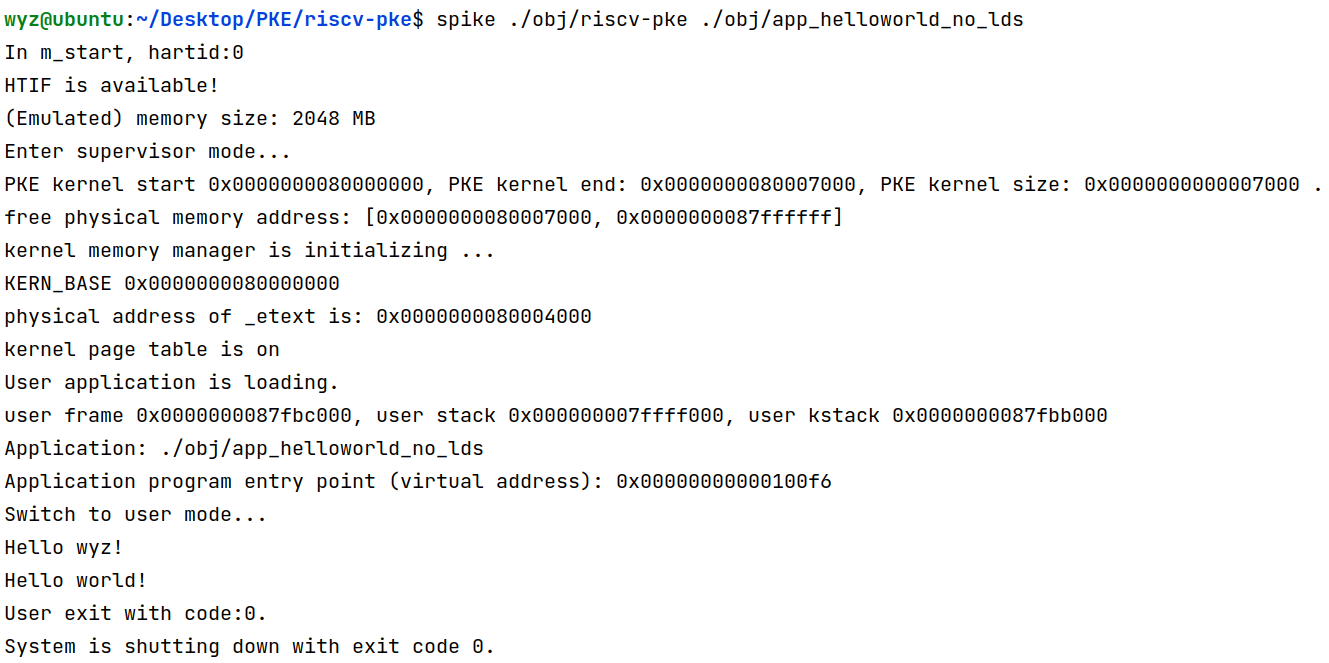
\includegraphics[width = 13cm]{figure/lab2_1_testresult.png}
    \caption{lab2_1虚实地址转换测试结果}
    \label{fig:lab2-1-testres}
\end{figure}

\paragraph{lab2_2 简单内存分配和回收}
简单内存分配和回收实验的测试程序如下所示。
% 图\ref{fig:lab1-2-testbench}
\begin{cppcode}
#include "user_lib.h"
#include "util/types.h"

struct my_structure {
  char c;
  int n;
};

int main(void) {
  struct my_structure* s = (struct my_structure*)naive_malloc();
  s->c = 'a';
  s->n = 1;
  printu("s: %lx, {%c %d}\n", s, s->c, s->n);
  naive_free(s);
  exit(0);
}
\end{cppcode}

编译运行测试程序,程序测试结果如图\ref{fig:lab2-2-testres}所示。程序打印了分配页面的起始虚拟地址和该页面中存放的结构体变量内容s: 0000000000400000, \{a 1\},随后以"0"作为退出码结束程序运行,说明简单内存分配和回收实验成功完成。

\paragraph{lab2_3 缺页异常}
缺页异常实验的测试程序如下所示,该程序使用递归函数的方式计算0到1000的所有整数和,由于函数的递归调用过程会产生较大的内存开销,故初始用户栈空间会被“压满”,程序需要多次执行缺页异常处理操作。

\begin{cppcode}
#include "user_lib.h"
#include "util/types.h"

uint64 sum_sequence(uint64 n) {
  if (n == 0)
    return 0;
  else
    return sum_sequence( n-1 ) + n;
}

int main(void) {
  uint64 n = 1000;
  printu("Summation of an arithmetic sequence from 0 to %ld is: %ld \n", n, sum_sequence(1000) );
  exit(0);
}
\end{cppcode}
\begin{figure}[!htbp]
    \centering
    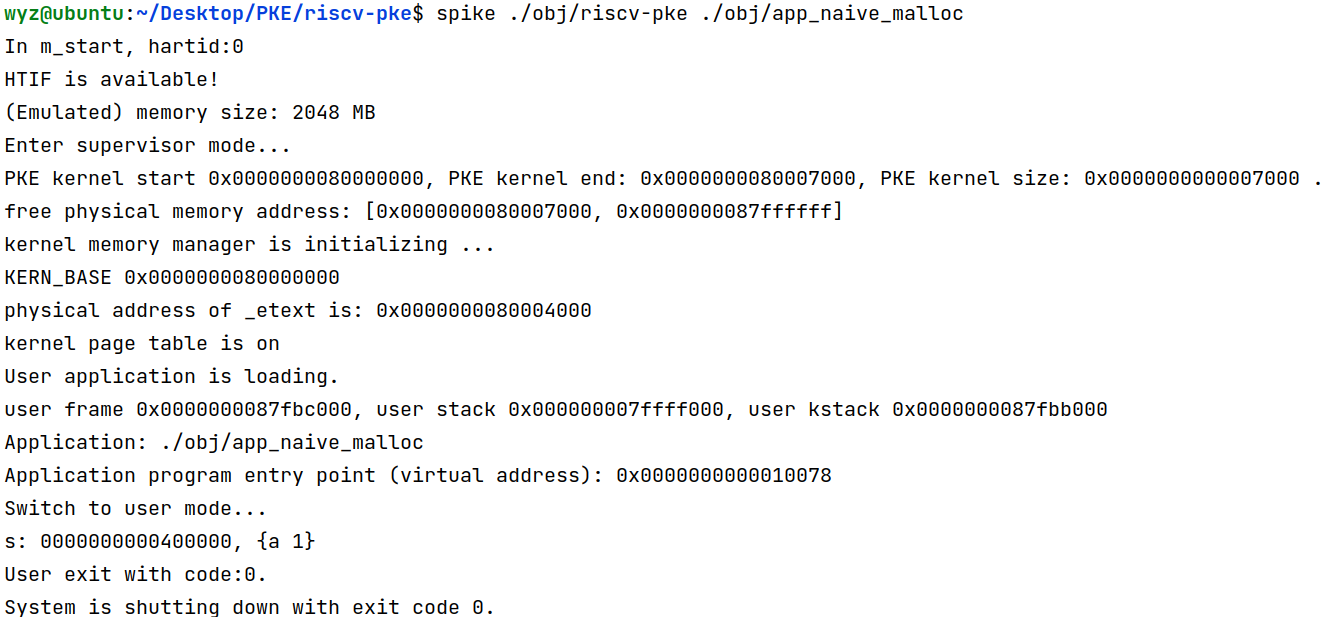
\includegraphics[width = 13cm]{figure/lab2_2_testresult.png}
    \caption{lab2_2简单内存分配和回收测试结果}
    \label{fig:lab2-2-testres}
\end{figure}
\begin{figure}[!htbp]
    \centering
    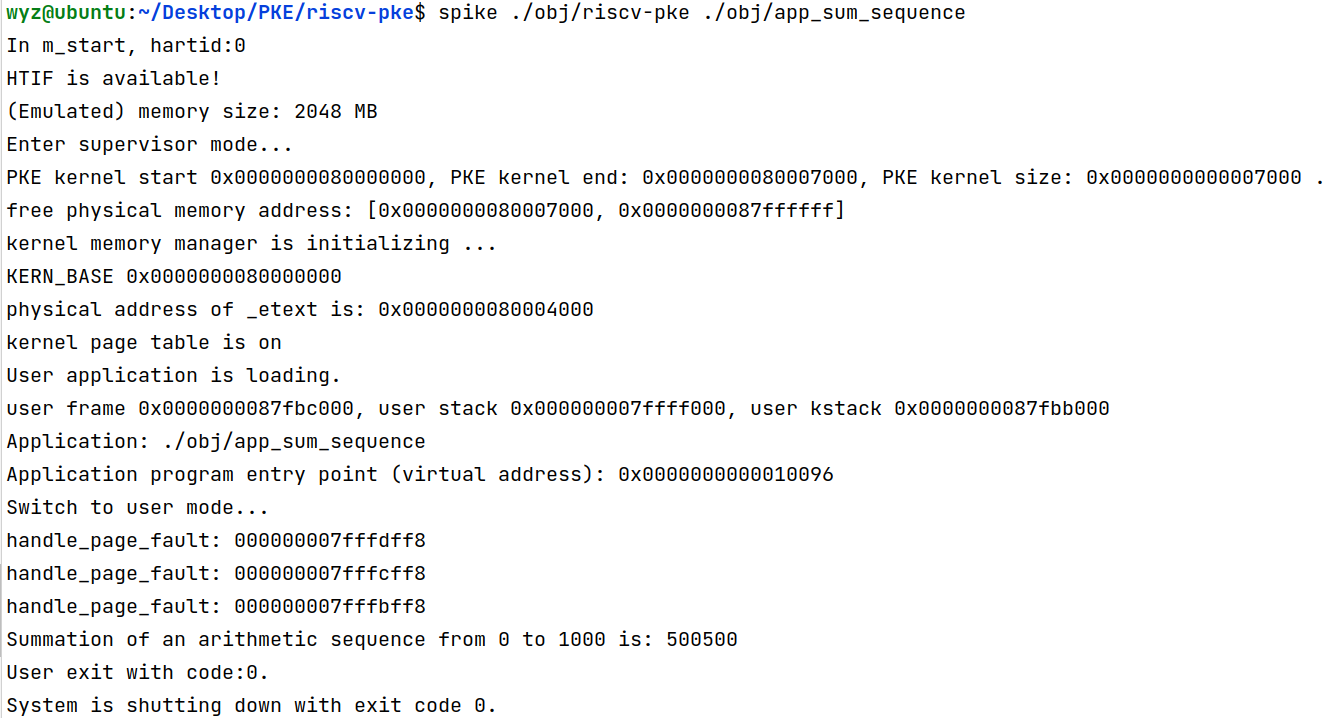
\includegraphics[width = 13cm]{figure/lab2_3_testresult.png}
    \caption{lab2_3缺页异常测试结果}
    \label{fig:lab2-3-testres}
\end{figure}

编译运行测试程序,程序测试结果如图\ref{fig:lab2-3-testres}所示,程序执行过程中执行了3次页错误处理,最终给出了正确的计算结果并正常退出,说明缺页异常实验成功完成。

\paragraph{lab2_challenge1 复杂缺页异常}
复杂缺页异常的测试程序如下。
\begin{cppcode}
#include "user_lib.h"
#include "util/types.h"

uint64 sum_sequence(uint64 n, int *p) {
  if (n == 0)
    return 0;
  else
    return *p=sum_sequence( n-1, p+1 ) + n;
}

int main(void) {
  uint64 n = 1037;
  int *ans = (int *)naive_malloc();
  printu("Summation of an arithmetic sequence from 0 to %ld is: %ld \n", n, sum_sequence(n+1, ans) );
  exit(0);
}
\end{cppcode}

该程序在缺页异常测试程序的基础上增加了动态分配的数组空间(起始地址为ans),由于页大小为4KB,且naive_malloc一次性分配一页内存空间,故ans指向的页可存放 $1024$ 个int类型的数据,因此当 $n$ 小于 $1024$ 时,程序正常运行;当 $n$ 超过 $1024$时 则会发生页面越界访问的问题,且为非法越界访问。

当$n$取值 $255$ 时,程序运行结果如图\ref{fig:lab2-c1-255}所示,经过两次缺页异常后程序返回了正常的结果并正常退出。
\begin{figure}[!htbp]
    \centering
    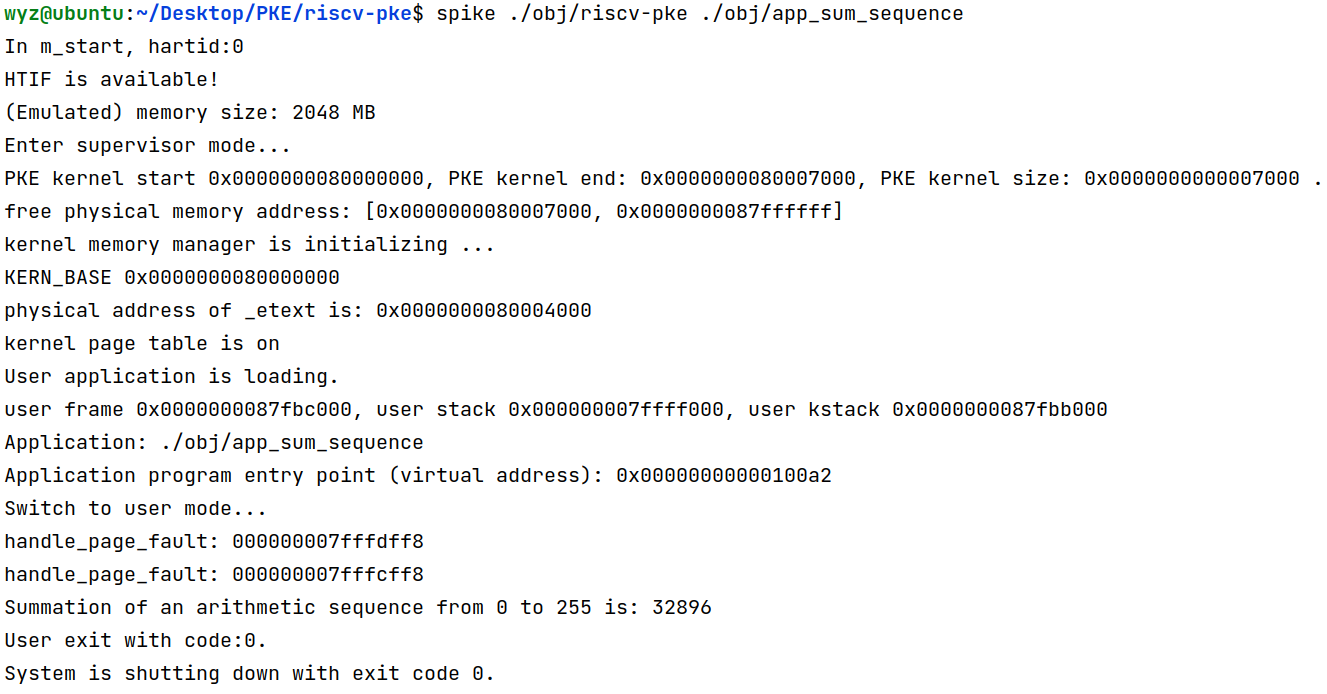
\includegraphics[width = 13cm]{figure/lab2_c1_testresult255.png}
    \caption{lab2_challenge1 n=255测试结果}
    \label{fig:lab2-c1-255}
\end{figure}

当$n$取值1037时,程序运行结果如图\ref{fig:lab2-c1-1037}所示。由于涉及堆空间越界访问,因此程序打印出错误信息并异常退出。
\begin{figure}[!htbp]
    \centering
    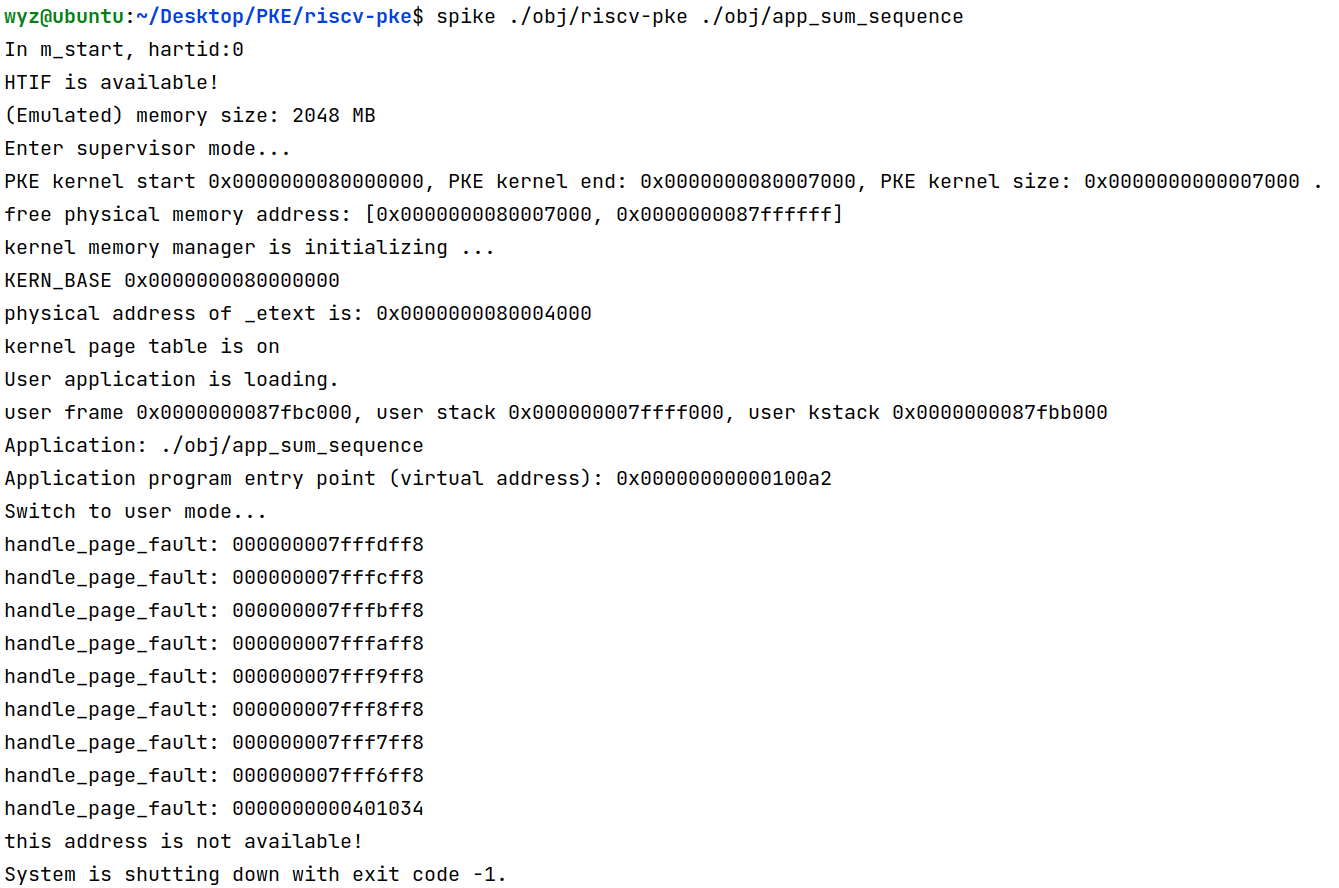
\includegraphics[width = 13cm]{figure/lab2_c1_testresult1037.png}
    \caption{lab2_challenge1 n=1037测试结果}
    \label{fig:lab2-c1-1037}
\end{figure}

两组实验结果表明,当前的异常处理程序已经可以正确处理栈空间不足引起的合法缺页异常和堆空间越界访问引起的非法缺页异常,达到了实验的要求。

\subsection{实验心得}
在此次实验中,我对操作系统的内存管理相关知识有了更加深入的理解与认识。

首先,我进一步理解并掌握了虚实地址转换机制的实现原理。我学习了PKE操作系统内核使用的Sv39虚地址管理方案,通过阅读相关的页表操作函数,对页表的处理原理有了实践层面的认知,并使用了合适的页表操作函数完成了S态下的虚实地址转换系统调用函数。

其次,我涉猎了较为简单的堆管理知识:简单的动态内存分配和回收机制。我阅读了实验中已经实现的naive_malloc函数,使用了合适的页表操作函数实现了naive_free系统调用的底层函数实现。

最后,我对简单和复杂情况下的缺页异常处理机制展开了探究,在handle_user_page_fault系统调用中,不仅处理了栈空间占满引发的合法缺页异常,还识别了堆空间越界访问引发的非法异常。

总之,这次实验让我在实践层面了解并掌握了操作系统内存管理的多种机制,收获颇为丰厚。
